\documentclass[8pt]{beamer}
\usepackage{tikz}
\usepackage[utf8]{vietnam}
\usepackage{amsmath}
\usepackage{graphicx}
\usepackage{wrapfig}
\usepackage{mathrsfs}
\usepackage{hyperref}
\usetheme{Copenhagen}
\usecolortheme{beaver}
\setbeamertemplate{navigation symbols}{}
\setbeamertemplate{headline}{}
\title[Chương 5: Biến đổi Z] %optional
{Chương 5: Biến đổi Z}
\subtitle{Tín hiệu và hệ thống}
\author[Tín hiệu và hệ thống] % (optional)
{Tín Vũ}
\date[VLC 2021] % (optional)
{tinvu1309@gmail.com}
\begin{document}
\frame{\titlepage}
\begin{frame}{Mục lục}
\tableofcontents
\end{frame}
\begin{frame}{Giới thiệu playlist}
\section{Giới thiệu playlist}
	\begin{itemize}
		\item Mình là Tín Vũ, hiện tại đang là sinh viên học tại Trường Đại học Công nghệ, Đại học Quốc gia Hà Nội. Mình tạo playlist video này để hỗ trợ các bạn học môn Tín hiệu và hệ thống trong các trường đại học kĩ thuật theo hướng \alert{trực quan hóa} nhất có thể.
		\item Do đó, mục tiêu của mình khi thực hiện playlist này không chỉ giúp các bạn ôn thi được điểm cao mà còn \alert{hiểu sâu công thức để làm nền tảng cho các môn học sau}.
		\item Để đạt được hai mục tiêu trên, các bạn nên xem \textbf{toàn bộ} video của mình, còn nếu chỉ cần ôn thi cấp tốc và đạt điểm cao thì hãy \textbf{bỏ qua} các video "optional".
		\item Nội dung playlist này chủ yếu bám sát nội dung môn học Tín hiệu và hệ thống tại trường của mình; nếu các bạn học trường khác, hãy tham khảo kĩ đề cương hay đề thi của trường bạn để đối chiếu sao cho ôn tập đúng trọng tâm và hợp lý. 
		\item Môn học này bao gồm \textbf{6} chương, các chương đều liên quan rất chặt chẽ và logic với nhau nên hãy học cẩn thận ngay từ \alert{chương 0} để ôn thi cuối kì đỡ vất vả.
	\end{itemize}
\end{frame}
\begin{frame}{Tài liệu tham khảo}
\section{Tài liệu tham khảo}
\begin{itemize}
		\item Tài liệu tham khảo chính: Signals and Systems (2nd edition) Alan V. Oppenheim and Alan S. Willsky.
		\item Tài liệu tham khảo phụ: Bài tập của mình học khóa trước, đề thi các năm cũ,...
		\item Tài liệu tham khảo phụ: Nếu bạn là sinh viên trường mình và muốn học "tủ" nhiều bài thì nên đọc Signals and Systems (2nd edition) Simon Haykin vì các thầy cô chủ yếu dạy và ra đề trong cuốn này, thế nhưng mình đánh giá cuốn này không đầy đủ và chi tiết như sách của Alan V. Oppenheim. 
	\end{itemize}
\end{frame}
\begin{frame}{Biến đổi Z}
\section{Khái niệm biến đổi Z}
\begin{itemize}
	\item Khái niệm biến đổi Z
\end{itemize}
Tương tự như biến đổi Laplace, biến đổi Z cũng là bài toán tìm vùng hội tụ (ROC) để tín hiệu rời rạc tồn tại biến đổi Fourier:
\begin{equation*}
\begin{split}
	X(z)=\sum_{n=-\infty}^{+\infty}x[n]\alert{{z}^{-n}}=\sum_{n=-\infty}^{+\infty}x[n](\alert{|r|e^{j\Omega})^{-n}}=\mathscr{F}(x[n]\alert{|r|^{-n}})
\end{split}
\end{equation*}
Nhân tử $|r|^{-n}$ có tác dụng "ép" tín hiệu rời rạc $x[n]$ về dạng tín hiệu năng lượng và cũng giống như biến đổi Laplace, ta mong muốn tìm tập giá trị của $|r|$ để $\mathscr{F}(x[n]\alert{|r|^{-n}})$ hội tụ.
\\Ví dụ: tìm biến đổi Z của tín hiệu rời rạc $x[n]=2^{n}u[n]$
$$X(z)=\sum_{n=-\infty}^{+\infty}x[n]z^{-n}=\sum_{n=0}^{+\infty}(2z^{-1})^n=\frac{1-(2z^{-1})^{+\infty}}{1-2z^{-1}}=\frac{1}{1-2z^{-1}}$$
Tổng vô hạn trên hội tụ khi và chỉ khi $|2z^{-1}|<1$, tương đương với $ROC:|z|>2$.
\\Suy ngẫm: tìm biến đổi Z của tín hiệu $x[n]=-2^{n}u[-n-1]$, nhận xét với kết quả trên.
\end{frame}
\begin{frame}{Biến đổi Z}
\section{Tính chất của biến đổi Z}
\begin{itemize}
	\item Tính chất của biến đổi Z
\end{itemize}
\begin{block}{Z transform pair}
\begin{equation*}
\begin{split}
	X(z)&=\sum_{n=-\infty}^{+\infty}x[n]z^{-n}\\
	x[n]&=\frac{1}{2\pi j}\oint_{C} X(z)z^{n-1}dz
\end{split}
\end{equation*}
\end{block}
Hoàn toàn tương tự như biến đổi Laplace, biến đổi Z ngược không sử dụng công thức (2) mà chỉ sử dụng bảng "Common Z transform pairs" kết hợp với tính chất để tìm tín hiệu gốc $x[n]$.\\ Ta sẽ xét một vài tính chất tiêu biểu của biến đối Z cùng với bảng "Common Z transform pairs".
\end{frame}
\begin{frame}{Biến đổi Z}
\begin{enumerate}
\item[1]  Dịch thời gian: $$\mathscr{Z}(x[n-n_{0}])=X(z)z^{-n}$$
\item[2]  Nhân mũ: $$\mathscr{Z}(a^{n}x[n])=X(za^{-1})$$
\item[3]  Lật tín hiệu: $$\mathscr{Z}(x[-n])=X(z^{-1})$$
\item[4] Đạo hàm trong miền Z: $$\mathscr{Z}(nx[n])=-z\frac{dX(z)}{dz}$$
\end{enumerate}
\begin{center}
\begin{tabular}{ |l|l| } 
 \hline
 $f[n]$ & $F(z)$ \\ 
 $\delta[n]$ & $1 \quad (ROC: \forall |z|)$ \\ 
 $u[n]$ &   $\frac{1}{1-z^{-1}} \quad (ROC: |z|>1)$ \\ 
 $a^n u[n]$ & $\frac{1}{1-az^{-1}}\quad (ROC: |z|>|a|)$\\
 $-na^n u[-n-1]$ & $\frac{1}{1-az^{-1}}\quad (ROC: |z|<|a|)$\\
 $a^{n}\cos(\Omega_{0}n)u[n]$ &$\frac{1-az^{-1}\cos{\omega_{0}}}{1-2az^{-1}\cos{\omega_{0}}+z^{-2} a^2}  \quad (ROC: |z|>|a|)$\\

 $a^{n}\sin(\Omega_{0}n)u[n]$ &$\frac{az^{-1}\cos{\omega_{0}}}{1-2az^{-1}\cos{\omega_{0}}+z^{-2} a^2}  \quad (ROC: |z|>|a|)$\\
 \hline
\end{tabular}
\end{center}
Suy ngẫm: hãy tự chứng minh lại toàn bộ các tính chất và công thức trên.
\end{frame}
\begin{frame}{Biến đổi Z}
\section{Phân tích hệ thống rời rạc}
\subsection{Phân tích tính chất của hệ thống rời rạc}
\begin{itemize}
\item Phân tích tính chất hệ thống rời rạc
\end{itemize}
Do mình rất bận nên không còn thời gian để phân tích kĩ biến đổi Z nữa, về mặt ý tưởng các bạn tự tham khảo \alert{Chương 4} để có cái nhìn bao quát về phân tích hệ thống bằng hệ điểm cực.
\begin{figure}[h]
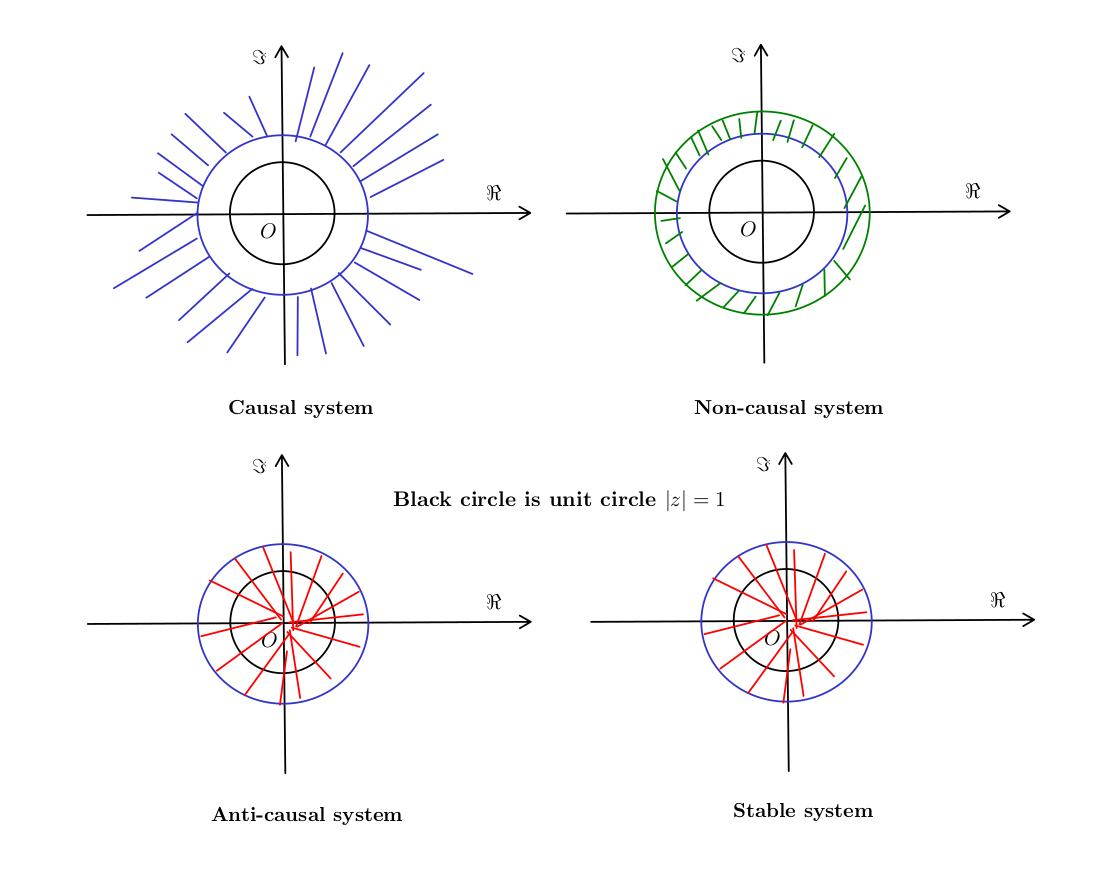
\includegraphics[width=0.7\textwidth]{z.jpg}
\caption{System properties}\label{fig:re1}
		\end{figure}
\end{frame}
\begin{frame}{Biến đổi Z}
\subsection{Phân tích đáp ứng hệ thống}
\begin{itemize}
	\item[-] Phân tích đáp ứng hệ thống rời rạc
\end{itemize}
Về ý tưởng, ta cũng định nghĩa phép biến đổi Z một phía (unilateral Z transform) như biến đổi Laplace một phía: $$\mathscr{X}(z)=\sum_{n=0}^{+\infty}x[n]z^{-n}=\mathscr{UZ}(x[n])$$ 
Ta cũng dùng biến đổi Z một phía để xét đáp ứng của hệ thống rời rạc có điều kiện khởi tạo:
$$\mathscr{UZ}(x[n-1])=\mathscr{X}(z)z^{-1}+x[-1]$$
$$\mathscr{UZ}(x[n-2])=\mathscr{X}(z)z^{-2}+x[-1]z^{-1}+x[-2]$$
\end{frame}
\end{document}
